% This is samplepaper.tex, a sample chapter demonstrating the
% LLNCS macro package for Springer Computer Science proceedings;
% Version 2.20 of 2017/10/04
%
\documentclass[runningheads]{llncs}
%
\usepackage{cite,url,amsfonts,amsmath}
\usepackage{algorithm}% http://ctan.org/pkg/algorithms
\usepackage{algpseudocode}% http://ctan.org/pkg/algorithmicx
\usepackage{mathtools}
\usepackage{graphicx}
\usepackage{color}
\usepackage{hyperref}
% Used for displaying a sample figure. If possible, figure files should
% be included in EPS format.
%
% If you use the hyperref package, please uncomment the following line
% to display URLs in blue roman font according to Springer's eBook style:
% \renewcommand\UrlFont{\color{blue}\rmfamily}
\DeclareMathOperator*{\argmin}{arg\,min}
\graphicspath{{figs/}, {../figures/}}

\begin{document}
%
\title{Artistic Curve Steganography Carried by Musical Audio}
%
%\titlerunning{Abbreviated paper title}
% If the paper title is too long for the running head, you can set
% an abbreviated paper title here
%
\author{First Author\inst{1}\orcidID{0000-1111-2222-3333}}
%
\authorrunning{F. Author et al.}
% First names are abbreviated in the running head.
% If there are more than two authors, 'et al.' is used.
%
\institute{Princeton University, Princeton NJ 08544, USA 
\email{lncs@springer.com}}
%
\maketitle              % typeset the header of the contribution
%
\begin{abstract}
The abstract should briefly summarize the contents of the paper in
15--250 words.

\keywords{Steganography, Traveling Salesperson Art, Hidden Signals}
\end{abstract}
%
%
%
\section{Introduction}



Our goals and design constraints are as follows:
\begin{enumerate}
    \item \label{goal:imperceptible} The hidden data should be audibly imperceptible
    \item \label{goal:geomquality} The hidden data should be faithfully preserved and {\em robust to compression}
    \item \label{goal:misalignment} The hidden data should be robust to frame misalignment, or it should be possible to recover a frame alignment without any prior information
    \item \label{goal:metadata} No metadata should be required to retrieve the hidden data; (compressed) audio alone should suffice
    \item \label{goal:partial} It should be possible to recover the data partially from partial audio chunks; that is, we don't need to wait for the entire data stream to recover the signal
\end{enumerate}

Goals ~\ref{goal:imperceptible} and ~\ref{goal:geomquality} are at odds with each other, and satisfying them simultaneously is the biggest challenge of this work.

Pipeline is simple enough that we have very good intuition for how it's working, and we validate its performance in Section~\ref{sec:experiments}.


\subsection{Prior Work in Audio Steganography}

\section{Traveling Salesperson Art}

\begin{figure}
  \centering
  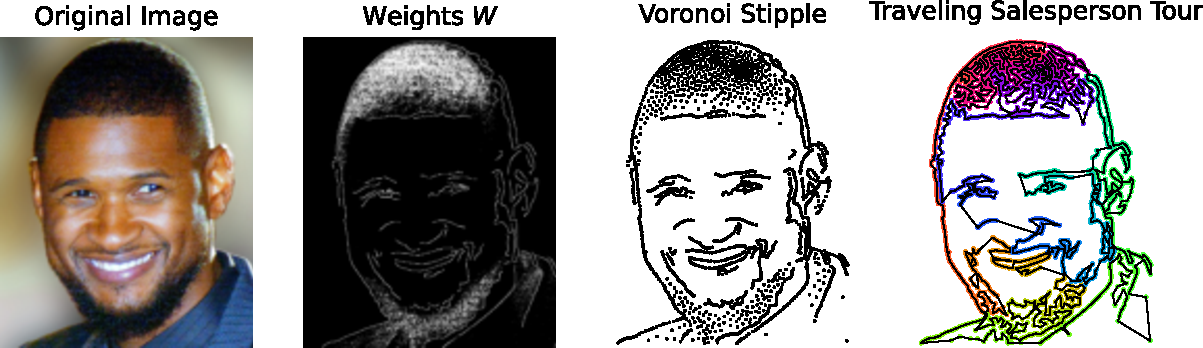
\includegraphics[width=\columnwidth]{TSPTour.pdf}
  \caption{Our modified pipeline for creating TSP art.  Color on the tour indicates phase along the loop.}
  \label{fig:TSPTour}
\end{figure}

Traveling Salesperson (TSP) art \cite{bosch2004continuous, kaplan2005tsp,bosch2008connecting} is an automated artistic line drawing pipeline which computes a {\em simple closed loop} to approximate a source image.  ``Simple'' in this context does not imply a lack of complexity; rather, it means that a curve does not intersect itself (see, for example, the Jordan Curve Theorem \cite{bosch2009jordan}).  To construct such a curve, we first place a collection of dots in the plane in a ``stipple pattern'' to approximate brightness in the image (e.g. more dots concentrate in darker regions), and then connect them in a loop via an approximate traveling salesperson (TSP) tour.  Figure~\ref{fig:TSPTour} shows an example.  We follow the TSP Art technique of \cite{kaplan2005tsp}, with a few modifications, as described below.


\subsection{Voronoi Stippling}
\label{sec:stippling}

\begin{algorithm}
  \caption{Modified Weighted Voronoi Stippling \cite{secord2002weighted}}
  \begin{algorithmic}[1]
    \Procedure{VoronoiStipple}{$G$, $N$, $b$, $\sigma$, $f$}
    \Comment{Grayscale image $G$, $N$ target points, brightness threshold $b$, Canny edge scale $\sigma$, density factor $f$}
    \State $W_{ij} \gets \min(I_{ij}, b)$
    \State $W_{ij} \gets W_{ij} - \min(W)$
    \State $W_{ij} \gets 1 - W_{ij} / \max(W)$
    \State $C \gets \text{canny}_{\sigma}(I)$ \Comment{1 if on canny edge, 0 otherwise}
    \State $W_{ij} \gets \max(W_{ij}, C_{ij})$
    \State  Sample $N$ random points $X \in \mathbb{R}^{N \times 2}$ by density according to $W$
    \For{$k = 1:10$} \Comment{Lloyd's relaxation iterations}
        \State \begin{equation}
          X_i \gets \frac{ \sum_{(i, j) \in A_i} W_{ij} * (i, j) }{\sum_{(i, j) \in A_i} W_{ij}}
        \end{equation}
        \Comment{Where $A_i$ is the Voronoi region for point $X_i$}
    \EndFor \\
    \State Remove top $N(1-f)$ points from $X$ with furthest distance to their nearest neighbors \\
    \Return $X$
    \EndProcedure
  \end{algorithmic}
  \label{alg:voronoistipple}
\end{algorithm}

%\begin{algorithm}
%  \caption{2-Opt Approximate TSP Tour \cite{johnson1997traveling}}
%  \begin{algorithmic}[1]
%    \Procedure{TSP2Opt}{$X$}
%    \Comment{$X \in \mathbb{R}^{N \times 2}$ is a 2D point cloud}
%    \State Let $T$ be a minimum spanning tree of $X$
%    \State Let $tour$ be indices into $X$ in the order that a depth-first search visits $T$, starting at an arbitrary point
%    \While{There exits a swappable $i > 1$, $j > i$}
%      \State Reverse indices in $tour$ in $[i+1, j]$
%    \EndWhile \\
%    \EndProcedure
%  \end{algorithmic}
%  \label{alg:twoopt}
%\end{algorithm}

The first step in TSP art is to generate a stipple pattern $X$ to best approximate a grayscale image $G$.  Following the authors of \cite{kaplan2005tsp}, we use Secord's technique for Voronoi stippling \cite{secord2002weighted}.  This consists taking an initial sample of points according to some density weights $W$ and then repeatedly moving them closer the weighted centroid of their Voronoi regions (an instance of Lloyd's algorithm) so that they are spread more evenly and look less ``noisy.''  Secord \cite{secord2002weighted} takes the weight $W_{ij}$ at a pixel to be inversely proportional to its brightness, using a weight of $0$ above some brigtness threshold $b$.  This leads more dots to concentrate in darker regions; however, the algorithm may fail to sample any dots along important edges between brighter regions (the authors of \cite{li2011structure} also observed this).   To ameliorate this, we run a Canny edge detector \cite{canny1986computational} on the original image and set the weight of any pixels along an edge to be 1, so that the final weights promote samples both in darker regions and along edges of any kind.  This addition is particularly helpful for line drawings, including images with text (e.g. Figure~\ref{fig:caltech101examples}).  Finally, we include the option to filter out points by density to clean up the stipple before the next step.  Algorithm~\ref{alg:voronoistipple} provides more details.

\subsection{Traveling Salesperson Tours}
\label{sec:tsp}
Once a stipple has been established, the next step in TSP art is to ``connect the dots'' with a closed loop that visits each stipple point exactly once, referred to as a ``tour''\footnote{A loop with these properties is otherwise known as a {\em Hamiltonian cycle} on a complete graph over the points}.  A well known objective function for a tour that doesn't ``jump too much'' is the total distance traveled, or the sum of all edge lengths, and a tour that achieves the optimum is known as a {\em traveling salesperson (TSP) tour}.  Since the TSP problem is NP-hard, the authors of  \cite{kaplan2005tsp} use the Concorde TSP solver \cite{applegate2001concorde} for an approximate solution. We opt for a simpler technique that first creates a 2-approximation of a TSP from a depth-first traversal through the minimum spanning tree of the stipple dots, which is a already a 2-approximation of the optimal tour.  We then iteratively improve on this tour via a sequence of 2-opt relaxations \cite{johnson1997traveling}; that is, if for some $i > 1, i < j < N$ the distances between the 4 points $X_i, X_{i+1}, X_j$, and $X_{j+1}$ satisfy


\begin{figure}
  \begin{minipage}[c]{0.6\textwidth}
    \caption{
      Every crossing in a tour can be removed with a 2-opt swap to yield a tour of a smaller distance, since, by the triangle inequality, $d(X_i, X_j) + d(X_{i+1}, X_{j+1}) < (a+d) + (b+c) = d(X_i, X_{i+1}) + d(X_j, X_{j+1})$.  This may introduce new crossings (shown in red), but these and other crossings will be resolved in future 2-opt swaps
    } \label{fig:TwoOpt}
  \end{minipage}
  \begin{minipage}[c]{0.38\textwidth}
    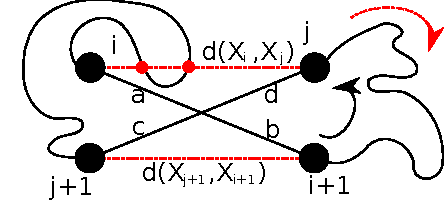
\includegraphics[width=\textwidth]{2Opt.pdf}
  \end{minipage}\hfill
  
\end{figure}

\begin{figure}
  \centering
  
  \caption{.}
  \label{}
\end{figure}

\begin{equation}
  d(X_i, X_j) + d(X_{i+1}, X_{j+1}) < d(X_i, X_{i+1}) + d(X_j, X_{j+1})
\end{equation}

then it is possible to perform a swap to yield a new tour with a smaller distance.  This amounts to reversing the indices in the tour between index $i+1$ and $j$, inclusive.  We repeat this step as long as such a swap is still possible.  Though this is not guaranteed to yield an optimal TSP tour, it does produce tours which are simple; that is, every crossing is removed (Figure~\ref{fig:TwoOpt}).


\subsection{Curvature Shortening Flow}

\begin{figure}
  \centering
  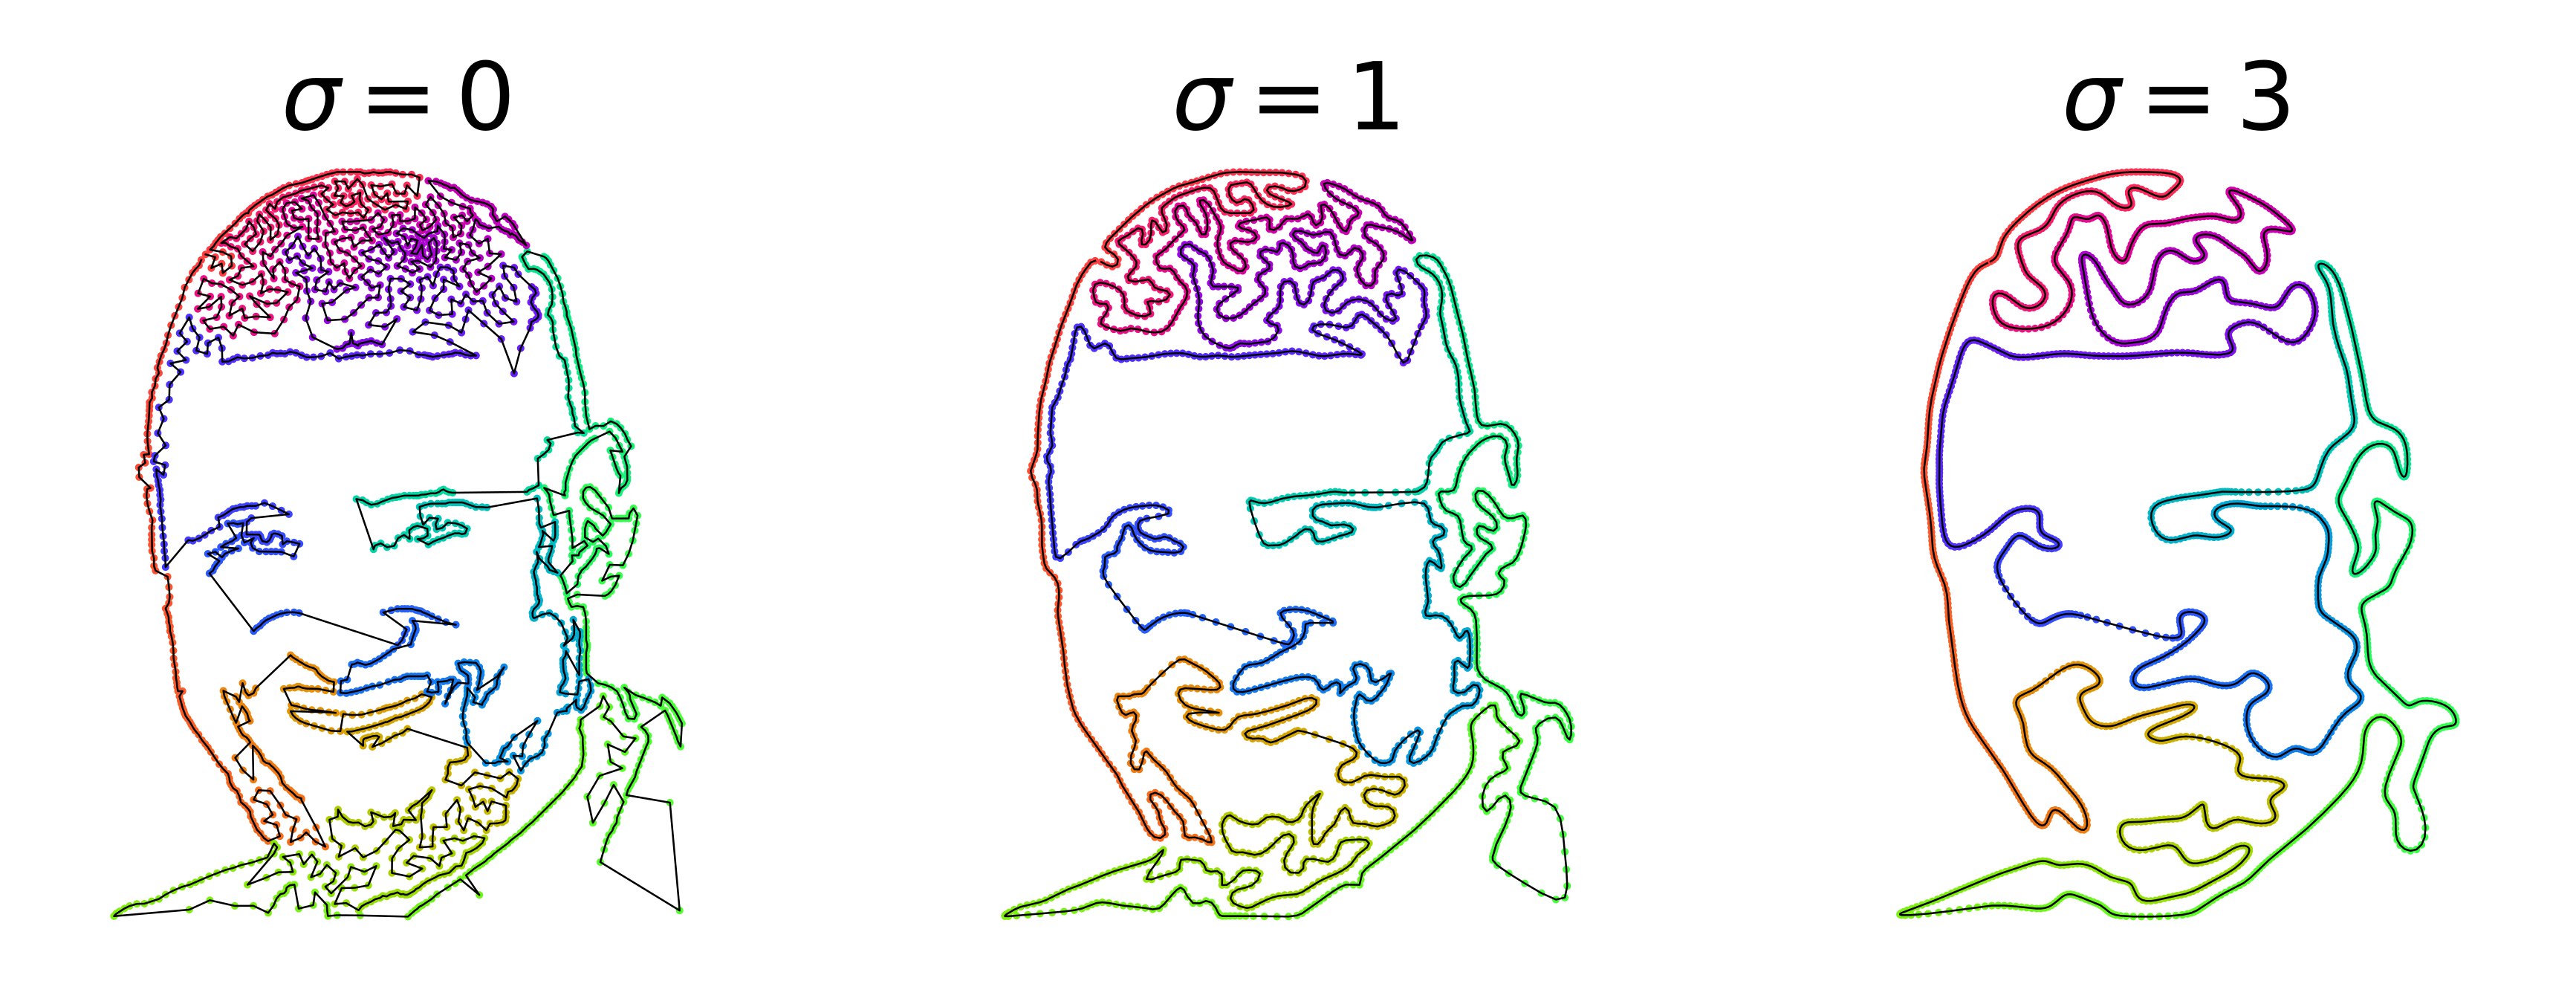
\includegraphics[width=\columnwidth]{CurvatureShortening.png}
  \caption{Anticipating that mp3 compression will introduce noise to our embedded curves, we pre-smooth them before hiding them using one iteration of curvature-shortening flow, which smooths the curves without introducing any crossings.  We find $\sigma=1$ to be a good tradeoff between smoothness and detail.}
  \label{fig:CurvatureShortening}
\end{figure}


Since mp3 compression introduces noise into our embedded curves, we smooth them before embedding to improve visual quality.  To this end, we apply a numerical version of curvature shortening flow described by Mokhtarian and Mackworth \cite{mokhtarian1992theory} which applies to piecewise linear curves (like our TSP tours).  The technique works by numerically by convolving coordinates of each curve with smoothed versions of Gaussians and their derivatives.  In particular, let 
\begin{equation}
  g_{\sigma}[j] = c_1 e^{-j^2 / (2 \sigma^2)}, 
  g'_{\sigma}[j] = - c_2 \frac{j}{\sigma^2} e^{-j^2 / (2 \sigma^2)}
\end{equation}

where $c_1$ and $c_2$ are appropriate normalization constants.  Then we estimate the arc length of a sampled curve $\gamma[j]$ with the rectangular integral of a smoothed velocity estimate:

\begin{equation}
  \label{eq:arclen}
  s_{\sigma}[j] = \sum_{k=1}^j |(\gamma * g'_{\sigma})[k]|
\end{equation}

To approximately smooth a curve via one step of curvature-shortening flow, Mokhtarian and Mackworth \cite{mokhtarian1992theory} show that it suffices to first re-parameterize by the arc length $s_{\sigma}$ in Equation~\ref{eq:arclen}, and then to smooth the curve by convolving with $g_{\sigma}$.  The beauty of convolving with Gaussians as such is that $\gamma$ does not even have to be differentiable, so this works on our piecewise linear TSP tours.  Furthermore, by the Gage-Hamilton-Grayson theorem, simple curves that undergo curvature shortening flow {\em remain simple} and eventually become convex, shrinking to a point under repeated applications of the flow.  Figure~\ref{fig:CurvatureShortening} shows an example of one application of curvature shortening flow for different $\sigma$ values.



\section{Hamiltonian Paths on Watertight Triangle Meshes}
\label{sec:hamiltonian}

\begin{figure}
  \centering
  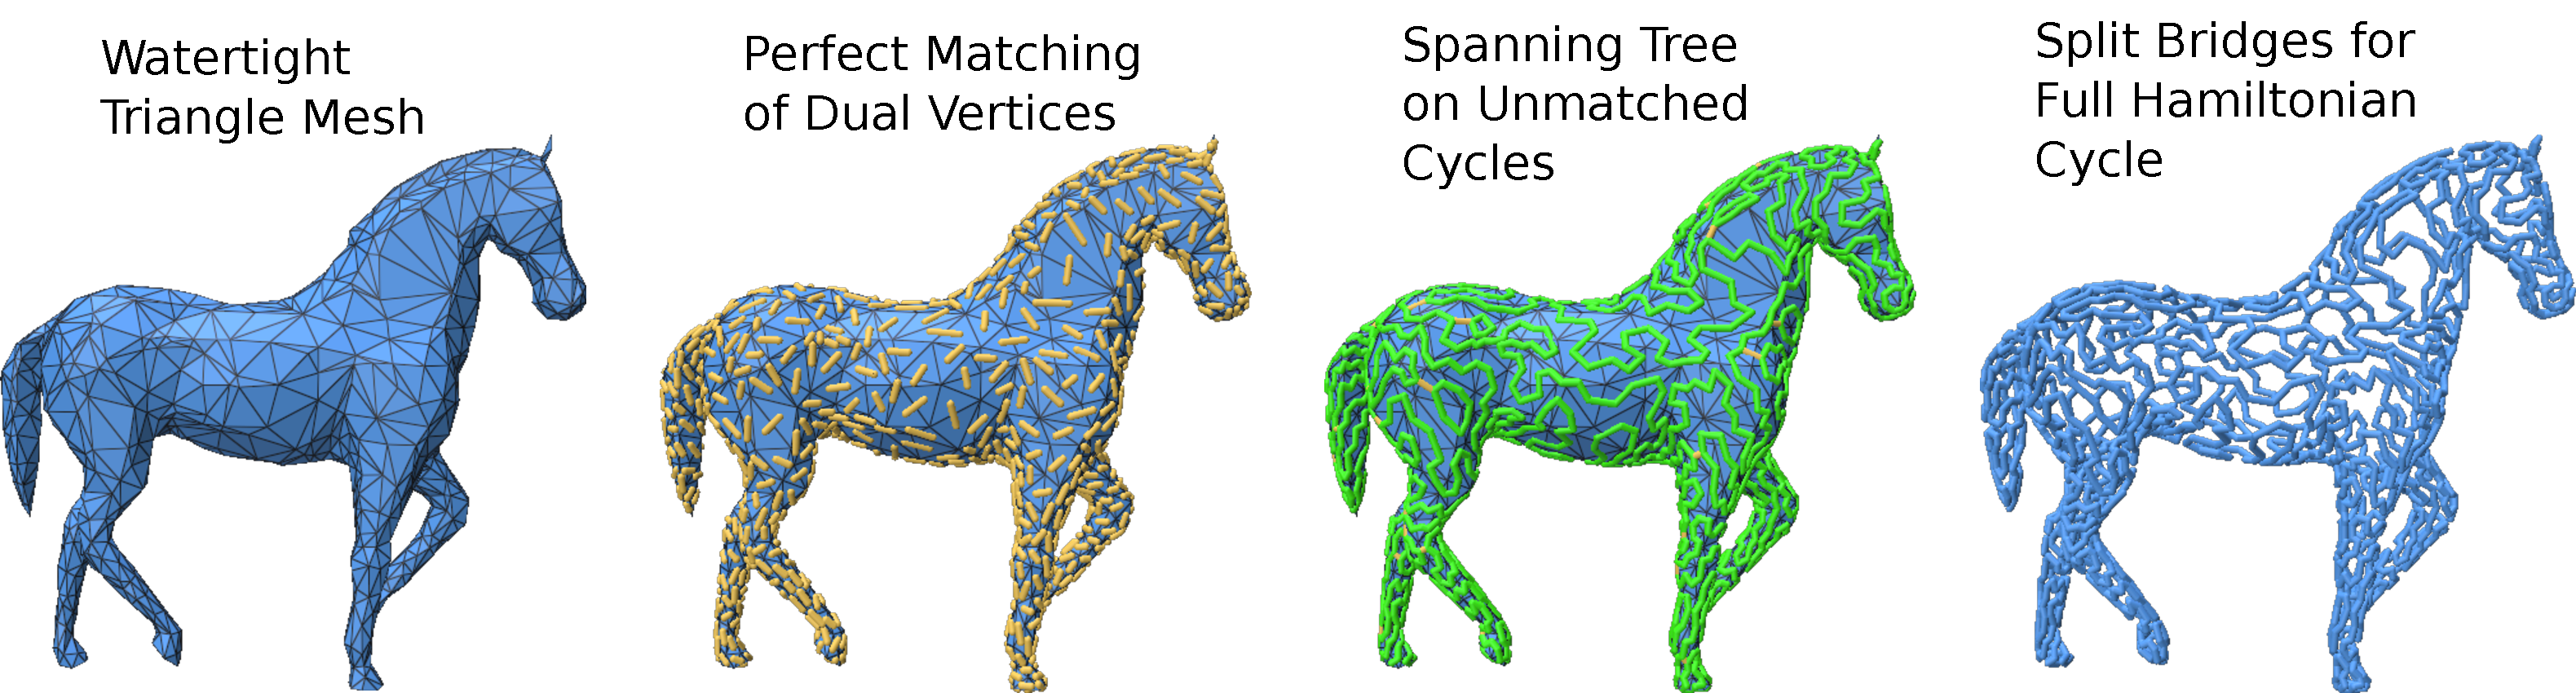
\includegraphics[width=\columnwidth]{HamiltonianHorse.pdf}
  \caption{An example of the algorithm of Gopi and Epstein \cite{gopi2004single} on a horse model from the Princeton mesh segmentation benchmark \cite{Chen:2009:ABF}.}
  \label{fig:HamiltonianHorse}
\end{figure}

In addition to 2D TSP tours on stipple patterns on planar images, we also create artistic 3D space curves that fill out the surfaces of 3D shapes following the technique of Gopi and Epstein \cite{gopi2004single}.  They observe that watertight triangle meshes (those with no boundary) have a dual graph in which a perfect matching exists.  In other words, it is possible to partition the triangles into a set of adjacent pairs (second column of Figure~\ref{fig:HamiltonianHorse}).  In practice, we use the Blossom-5 algorithm \cite{kolmogorov2009blossom} to find perfect matches of the dual graph.  Then, adding edges between unpaired triangles leads to a set of disconnected cycles (third column of Figure~\ref{fig:HamiltonianHorse}), which are connected by a spanning set of edges between paired triangles.  Finally, the spanning edges are split into bridges between the disconnected cycles, joining them together into one large cycle that covers the surface of the triangle mesh.


\section{Curve Embedding in Audio}

We now introduce our new algorithm for hiding artistic space curves, such as 2D TSP paths (Section~\ref{sec:tsp}) and 3D Hamiltonian paths (Section~\ref{sec:hamiltonian}), in audio.  Before we go into the details, we first define quantitative measurements for measuring the fit to the original audio (Goal~\ref{goal:imperceptible}) and the geometric quality of the hidden curve (Goal~\ref{goal:geomquality}).  Let the original carrier audio be $x$ and let the steganography audio be $y$, each with $N$ samples.  Then we define the steganographic signal to noise ratio in decibels (dB) as 

\begin{equation}
  \label{eq:stegsnr}
   \text{snr}(y|x) = 10  \log_{10} \left(\sum_{j=1}^N x_j^2 \right) -  10 \log_{10}\left(\sum_{j=1}^N (y_j-x_j)^2  \right)
\end{equation}

For our geometric measurement of quality, let $X_i$ be a sequence of $M$ target curve points in $\mathbb{R}^d$ and $Y_i$ be a sequence of $M$ reconstructed points in $\mathbb{R}^d$.  Then we define the {\em mean geometric distortion} is simply as the mean Euclidean distance between these points 

\begin{equation}
  \label{eq:distortion}
  \text{distortion}(Y|X) = \frac{1}{M} \sum_{j=1}^M ||X_j - Y_j||_2
\end{equation}


\subsection{Formulation of Least Squares Problem}

We now formulate an objective function that trades off Equation~\ref{eq:stegsnr} and Equation~\ref{eq:distortion}.  Let $T = (T_1, T_2, \hdots, T_N \}$ be the sequence of points of the target curve to hide, where each $T_i \in \mathbb{R}^d$, and let $T_{i, m}$ refer to $m^{\text{th}}$ coordinate of $T_i$, and let $x$ be a set of audio samples which will serve as a carrier.  The goal is to perturb the samples of $x$ so that some function of $x$ matches $T$ as closely as possible.  The function we choose is based on a ``time regularized'' version of the magnitude Short-Time Fourier Transform (STFT) which we call a {\em sliding window sum} STFT (SWS-STFT).  As a first step, we compute a {\em non-overlapping} STFT $S$ based on a chosen window length $w$ with a total of $N$ frames:

\begin{equation}
  S_{k, j} = \sum_{n = 0}^w x_{jw + n} \left(e^{-i 2 \pi k n / w} \right) = M_{k, j} \left( e^{i P_{k, j}} \right)
\end{equation}

and we factor $S$ it into its magnitude and phase components $M$ and $P$, respectively.  Next, we choose a subset of $d$ frequencies $k_i$, each of which will hide a different dimension of $T$.  Given a second window length $\ell$, we then define the following {\em sliding window sum} function, which we apply to each row $k_i$ of the magnitudes of $S$ that we wish to perturb to obtain the SWS-STFT

\begin{equation}
  \text{SWS}^{\ell}(M)_{k_i, j} = \sum_{n = 0}^{\ell-1} M_{k_i, j+n}
\end{equation}

The effect of $\ell$ is to smooth out the noisy rows $k_i$ of the magnitude spectrogram so that the rows in the SW-STFT match smoother transitions in the target curves.  Each row of the SW-STFT has $N-\ell+1$ samples.  Let's assume momentarily that $T$ has exactly this many samples; we will address the case where $\text{length}(T) > N-\ell+1$ in Section~\ref{sec:reparam}.  We then seek a perturbed version of the magnitudes $\hat{M}$ so that each coordinate $i$ is hidden in a single frequency index $k_i$ of $\hat{M}$.  To that end, we minimize the following objective function, one coordinate dimension $i = 1, ... d$ at a time:

\begin{equation}
  \label{eq:objfn}
  f(\hat{M}_{k_i}) = \sum_{j=1}^{N-\ell+1} \left( \left( \sum_{n = 0}^{\ell-1} \hat{M}_{k_i, j+n} \right) - T_{i, j} \right)^2 + \lambda \sum_{j=1}^N \left( M_{k_i, j} - \hat{M}_{k_i, j} \right)^2
\end{equation}



\begin{figure}
  \centering
  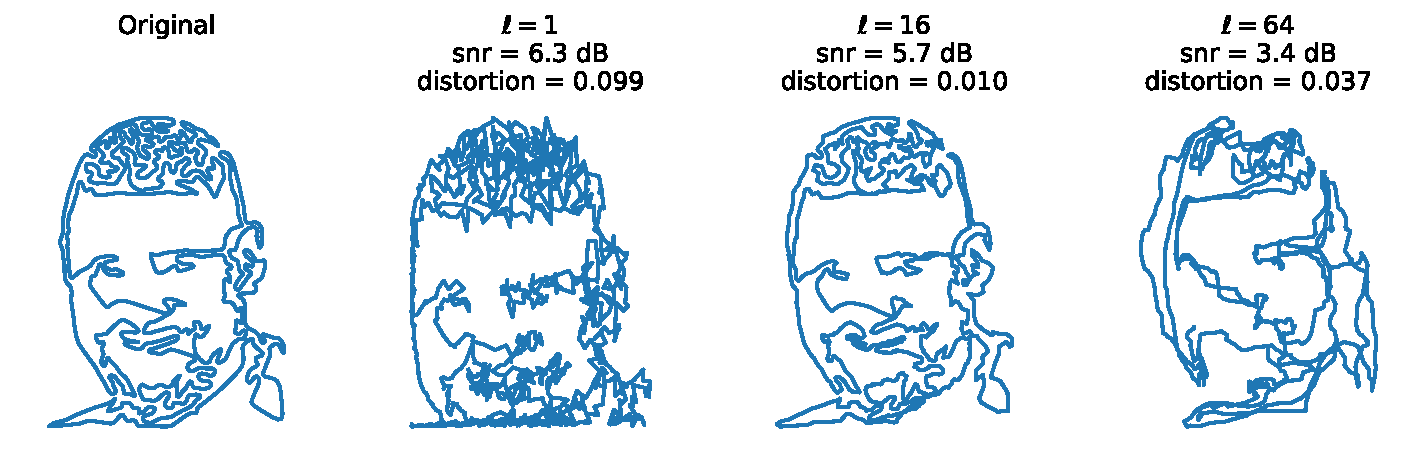
\includegraphics[width=\columnwidth]{WindowEffect.pdf}
  \caption{This figure shows the effect of varying $\ell$ for a fixed $\lambda=0.1$, using the lowest two non-DC frequencies to embed each coordinate.  A larger $\ell$ for the SW-STFT in Equation~\ref{eq:objfn} leads to smoother curves which are more likely to survive compression, but an $\ell$ that's too large may over-smooth.}
  \label{fig:WindowEffect}
\end{figure}

\begin{figure}
  \centering
  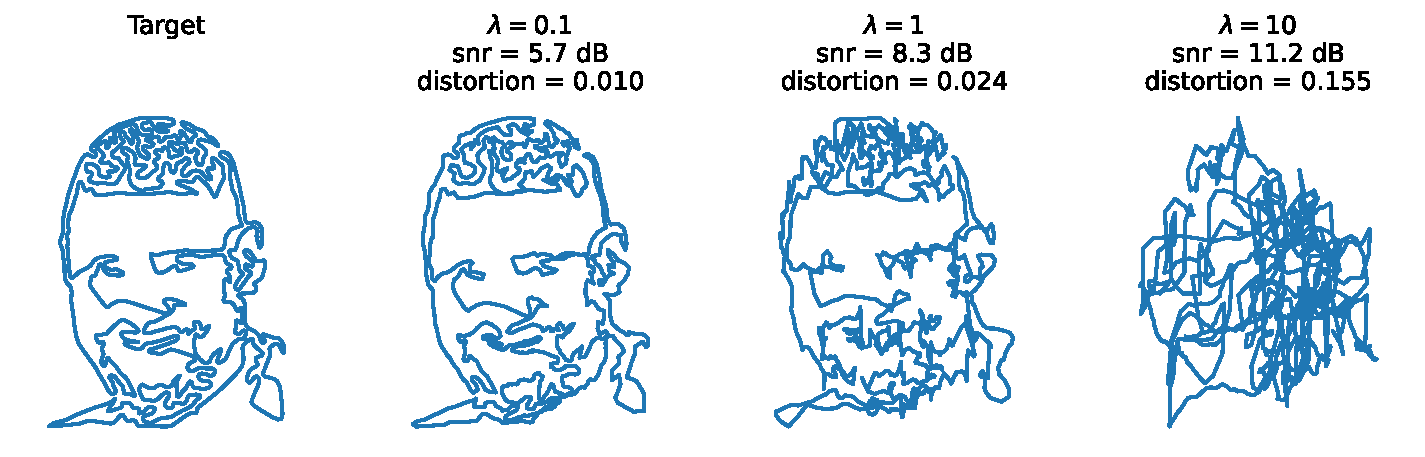
\includegraphics[width=\columnwidth]{LambdaEffect.pdf}
  \caption{This figure shows the effect of varying $\lambda$ for a fixed $\ell=16$, embedding using the lowest two non-DC frequencies to.  A smaller $\lambda$ in Equation~\ref{eq:objfn} leads to higher geometric fidelity (Goal~\ref{goal:geomquality}), at the cost of audio quality (Goal~\ref{goal:imperceptible}), as measured by SNR.}
  \label{fig:LambdaEffect}
\end{figure}



subject to $\hat{M_{k_i, j}} \geq 0$.  In other words, we want the magnitude SW-STFT of a perturbed signal to match the target coordinate as well as possible (minimizing Equation~\ref{eq:distortion}), while preserving the original audio as well as possible (minimizing Equation~\ref{eq:viterbiobj}), according to $\lambda$.  A greater $\lambda$ means that the signal will fit the original audio better, at the cost of a noisier curve.  Figure~\ref{fig:LambdaEffect} shows an example.

After solving for $\hat{M_{k_i, j}}$, we replace all rows of $M_{k_i}$ with $\hat{M_{k_i}}$, and we perform an inverse STFT of $M e^{i P}$ for the original phases $P$ (Section~\ref{sec:componentscales} will explain when it is necessary to modify the phases as well).  We then save the resulting audio in a compressed format, and recover the hidden signal by loading it in and extracting the corresponding components of the magnitude SW-STFT.


\subsubsection{Computational Complexity}
\label{sec:computation}
Minimizing equation~\ref{eq:objfn} can be formulated as a sparse nonnegative linear least squares problem, and there are myriad algorithms (e.g. \cite{branch1999subspace}) for solving such systems efficiently via repeated evaluation of the linear system and its adjoint on iterative estimates of a solution .  Furthermore, though Equation~\ref{eq:objfn} suggest an $O(N \ell)$ time complexity to evaluate the objective function at each iteration, we implement the linear operator and its adjoint with $O(N)$ operations only, independent of $\ell$, using the 1D version of the ``summed area tables'' trick in computer vision \cite{lewisfast}.  For example, let $C_{k_i, j} = \sum_{i=0}^{j} \hat{M_{k, i}}$, and $C_{k_i, j < 1} = 0$.  Then Equation~\ref{eq:objfn} can be rewritten as 
\begin{equation}
  \label{eq:objfncumusum}
  f_i(\hat{M}) = \sum_{j=1}^{N-\ell+1} \left( (C_{k_i, j+\ell-1}-C_{k_i, j-1}) - T_{i, j} \right)^2 + \lambda \sum_{j=1}^N \left( M_{k_i, j} - \hat{M}_{k_i, j} \right)^2
\end{equation}


It is also worth noting that a higher $\lambda$ in equation~\ref{eq:objfn} leads to a lower condition number\footnote{The condition number of a matrix is defined as the ratio of the largest to smallest singular values, and lower condition numbers are more numerically desireable.} of the matrix in the implied linear system, which leads to faster minimization of Equation~\ref{eq:objfn}.  But as Figure~\ref{fig:LambdaEffect} shows, it may still be worth it to use smaller $\lambda$ values.  In practice, we see it as a difference between an encoding in 30 seconds of audio that takes a few seconds for $\lambda=0.1$ versus an encoding that takes a split second for $\lambda=10$ on a CPU.



\subsubsection{The choice of non-overlapping windows}
Though some other works use transforms with overlapping windows \cite{hwan_sik_yun_acoustic_2010,geleta_pixinwav_2021}, changing different STFT bins independently leads to STFTs that do not correspond to any real signal due to discrepancies between overlapping windows.  An algorithm like Griffin-Lim \cite{griffin1984signal} can recover a signal whose spectrogram has a locally minimal distance to the perturbed STFT, but we find that this step introduces an unacceptable level of distortion both in the target and the carrier audio.  This problem occurs even for real-valued transforms such as the Discrete Cosine Transform (which was used by \cite{geleta_pixinwav_2021}).  Like \cite{xiaoxiao_dong_data_2004}, we sidestep this problem by using non-overlapping windows.  

Aside from window effects, the main downside of non-overlapping windows is that they lead to fewer STFT frames.  For instance, with a 30 second audio clip at 44100hz using a window length of 1024, we are limited to about 1292 frames, which is half of what we would get using an overlapping STFT with a hop length of 512.  However, a quick thought experiment shows that this is still a reasonable data rate.  Suppose that we use a sliding window length $\ell=16$, for a total of 1277 carrier samples.  Suppose also that the precision of our embedding of a 2D plane curve is roughly on par with an 8 bit per coordinate quantization in a more conventional binary encoding scheme.  Then the total number of bits transmitted over 30 seconds is $1277 \times 8 \times 2$, or about 681 bits/second.  This number jumps to about 1022 bits/second for a 3D curve.  These numbers are on par with other recent techniques that are designed to be robust to noise (e.g. 900 bits/second in the OFDM technique of \cite{eichelberger_receiving_2019}).  Furthermore, our equivalent of a ``bit error'' is additive coordinate noise, and the hidden signal degrades continuously with increased noise, rather than reaching a failure mode when a bit error is too high.




\subsection{Shifting, Scaling And Re-Parameterizing Targets for Better Fits}
\label{sec:reparam}

In this section, we explain how to modify the target curves to better match the given SW-STFT so that the STFT magnitudes don't have to be perturbed as much for the SW-STFT to match the target, leading to a less noticeable embedding of the hidden curve for the same quality geometry.

\subsubsection{Vertical Translation/Scaling}

A crucial step to keep the hidden signal imperceptible is to shift and rescale the target coordinates of the hidden curve to match the dynamic range of the SW-STFT components.  We first choose a scale ratio $a_i$ for each component as the ratio of the standard deviations $\text{stdev}_j \left( \text{SWS}^{\ell} (M)_{k_i, j} \right) / \text{stdev}_j (T_{i, j})$.  Then, letting $N$ be the length of the two signals, we compute the vertical shift $b_i$ as

\begin{equation}
  b_i = \frac{1}{N} \sum_{j=1}^N  \text{SWS}^{\ell} (M)_{k_i, j} - a_i T_{i, j}
\end{equation}

The rescaled target coordinate $\hat{T_i}$ is then defined as $\hat{T}_{i, j} = a_i T_{i, j} + b_i$.  Unfortunately, we lose relative scale information between the components, but we will explain how to hide and recover this in Section~\ref{sec:componentscales}

\subsubsection{Viterbi Target Re-Parameterization}


\algrenewcommand\algorithmicindent{0.8em}%
\begin{algorithm}
  \caption{Viterbi Target Re-Parameterization}

  \begin{algorithmic}[1]
    \Procedure{ViterbiTargetReparam}{$\hat{T}$, $\text{SWS}^{\ell} (M)$, $K$}
    \State $N_T \gets \text{len}(\hat{T})$ \Comment{Number of target points}
    \State $N_M \gets \text{len}(\text{SWS}^{\ell}(M))$ \Comment{Number of SW-STFT frames}
    \State $S[i>1, j] \gets 0$ \Comment{$N_T \times N_M$ Cumulative cost matrix}
    \State $S[1, j] \gets \sum_{i=1}^d (\hat{T}_{i, 1} - \text{SWS}^{\ell} (M)_{k_i, j})^2$
    \State $B[i, j] \gets 0$ \Comment{$N_T \times N_M$ backpointers to best preceding states}
    \For{$j = 2:N_M$}
        \For{$t = 1:N_T$}
            \State $S[t, j] = \min_{k=(t-K) \mod N_T} ^ {k=(t-1) \mod N_T} S[k, j-1] $ \Comment {Find best preceding state}
            \State $S[t, j] \gets S[t, j] + \sum_{i=1}^d (\hat{T}_{i, t} - \text{SWS}^{\ell} (M)_{k_i, j})^2$ \Comment{Add on matching cost}
            \State $B[t, j] = \argmin_{k=(t-K) \mod N_T} ^ {k=(t-1) \mod N_T} S[k, j-1] $ \Comment {Save reference to best preceding state}
        \EndFor
    \EndFor
    \State Backtrace $B$ to obtain the optimal sequence $\Theta$ \\
    \Return $\Theta$
    \EndProcedure
  \end{algorithmic}
  \label{alg:viterbiwarp}
\end{algorithm}

Beyond shifting and scaling the targets coordinates vertically, we may also need to re-parameterize them in time, since, in general, the SWS-STFT sequence will not have the same number of samples as the shifted target $\hat{T}$.  Furthermore, the target curves are cyclic, so the starting point is arbitrary, nor does it matter if we traverse the curve left or right.  This gives us a lot of freedom in how we choose to re-parameterize the target to best match the signal even before we perturb the signal.  Let $N_M$ be the number of frames in the SW-STFT and $N_T$ be the number of samples of the target, and assume that $N_T > N_M$ (we can always resample our target curves to make this true).  Let $\Theta = \{ \theta_1, \theta_2, \theta_3, \hdots, \theta_{N_M} \}$ be new indices into the target, and let $K > 0$ be a positive integer so that $1 \leq \left( (\theta_i - \theta_{i-1}) \mod N_T \right) \leq K$; that is, $K$ is the maximum number of samples by which the target re-parameterization can jump in adjacent time steps.  We seek a $\Theta$ minimizing the following objective function for a $d$-dimensional shifted target $\hat{T}$

\begin{equation}
  \label{eq:viterbiobj}
  g(\Theta = \{\theta_1, \theta_2, \hdots, \theta_{N_M}\}) = \sum_{j = 1}^{N_M} \sum_{i=1}^d \left( \text{SWS}^{\ell} (M)_{k_i, j} - \hat{T}_{i, j}  \right)^2
\end{equation}

For a fixed $K$, we use the Viterbi algorithm to obtain a $\Theta$ minimizing Equation~\ref{eq:viterbiobj} in $O(MNK)$ time.  Our use of the Viterbi algorithm for re-parameterizing geometric sequences is similar to the technique for corpus-based concatenative synthesis presented by the authors of \cite{schwarz2007corpus}.  Algorithm~\ref{alg:viterbiwarp} gives more details.  

\begin{figure}
  \centering
  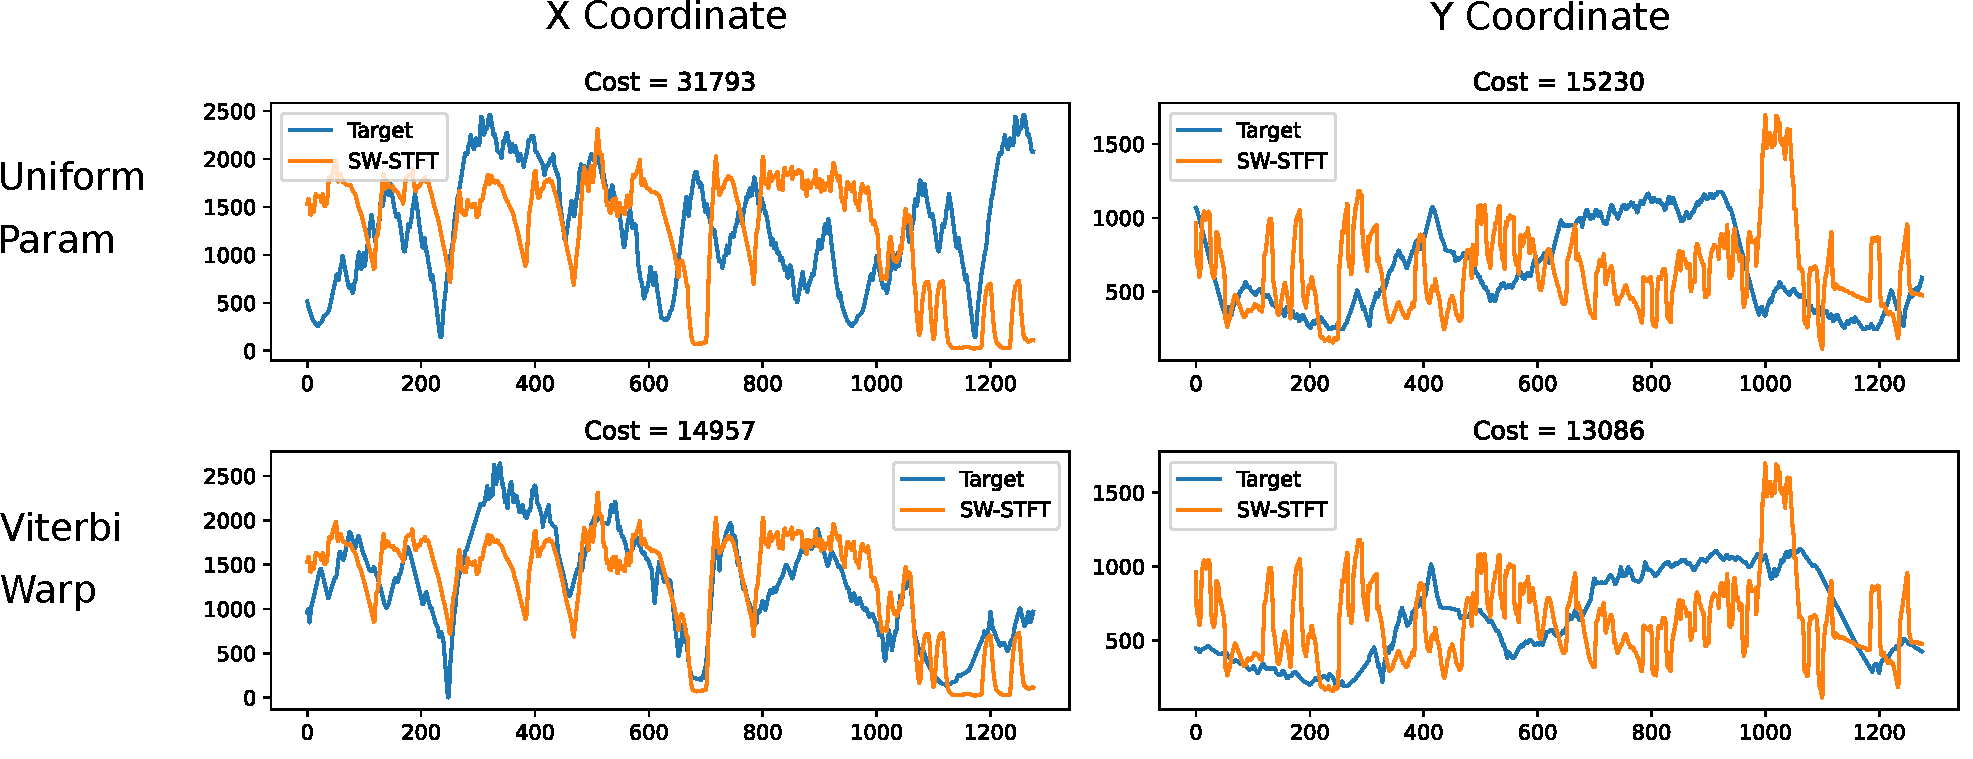
\includegraphics[width=\columnwidth]{Viterbi.pdf}
  \caption{Circularly shifting the target loop and traversing it at a non-uniform speed traces out the same shape, while matching the given SW-STFT better than a uniform parameterization starting at an artibrary place on the target.}
  \label{fig:ViterbiWarp}
\end{figure}

In practice, we re-run the algorithm starting at $K = 1$, and we repeatedly increment $K$ until the optimal $\Theta$ goes through at least one full loop on the target.  Since clockwise or counter-clockwise traversal of the target is arbitrary, we then rerun this procedure again for a reversed version of the sequence and keep the result which minimizes Equation~\ref{eq:viterbiobj}.  As a rule of thumb, we find that having a target curve with about 1.5-2x as many samples as there are SWS-STFT frames gives enough wiggle room for the Viterbi algorithm.  In our experiments in Section~\ref{sec:experiments}, we will generate TSP and Hamiltonian sequences with 2000 samples for our 1200-1300 SWS-STFT frames.  Figure~\ref{fig:ViterbiWarp} shows an example running this algorithm under these conditions on the Usher example in column 3 of Figure~\ref{fig:WindowEffect}.







\subsection{Storing Component Scales in Phase}
\label{sec:componentscales}

We use the technique presented by the authors of \cite{xiaoxiao_dong_data_2004} to recover the scales of each component.

\subsection{Recovering Frame Alignments}

\begin{figure}
  \centering
  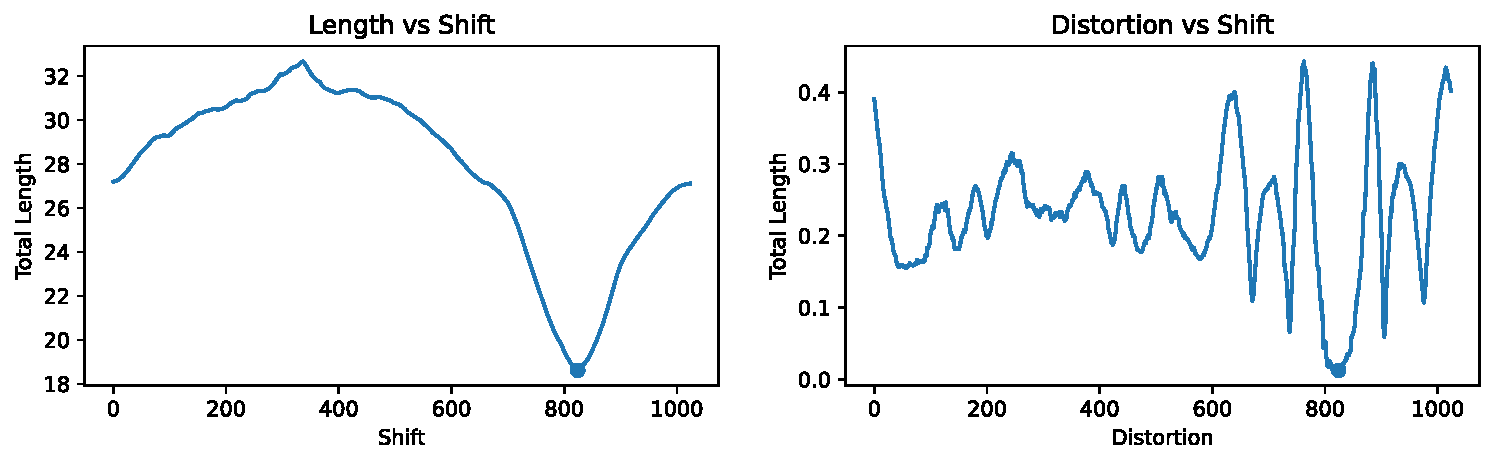
\includegraphics[width=\columnwidth]{OptimalShift.pdf}
  \caption{A shift which minimizes curve length is most likely the shift needed to re-align audio to frame windows.  The dot here indicates the ground truth shift of an embedding using the lowest two non-DC frequencies with $\lambda=0.1, \ell=16$, and the global mins exactly match ground truth.}
  \label{fig:FrameAlignments}
\end{figure}

What we've described so far works for audio that is aligned to each window, but additional work needs to be done to address Goal ~\ref{goal:misalignment} if the audio to decode comes in misaligned.  To this end, we use the fact that the hidden curves move only slightly between adjacent samples; a TSP tour is defined as length-minimizing, and adjacent samples in Hamiltonian cycles on meshes move only between neighboring triangles on the original mesh.  If the embedding is frame aligned, the length of the curve should be minimized.  Conversely, if the embedding is not frame aligned, the curve becomes noisy and is more likely to jump around quickly from sample to sample.  Therefore, we can pick the alignment which minimizes the length in all possible shifts from $0$ to $win$.  Figure~\ref{fig:FrameAlignments} shows an example.  We will empirically evaluate this in Section~\ref{sec:experiments}.





\section{Experiments}
\label{sec:experiments}

Below we assess the performance of our system on an extensive set of tests

Show caltech-101 and meshseg examples

\begin{figure}
  \centering
  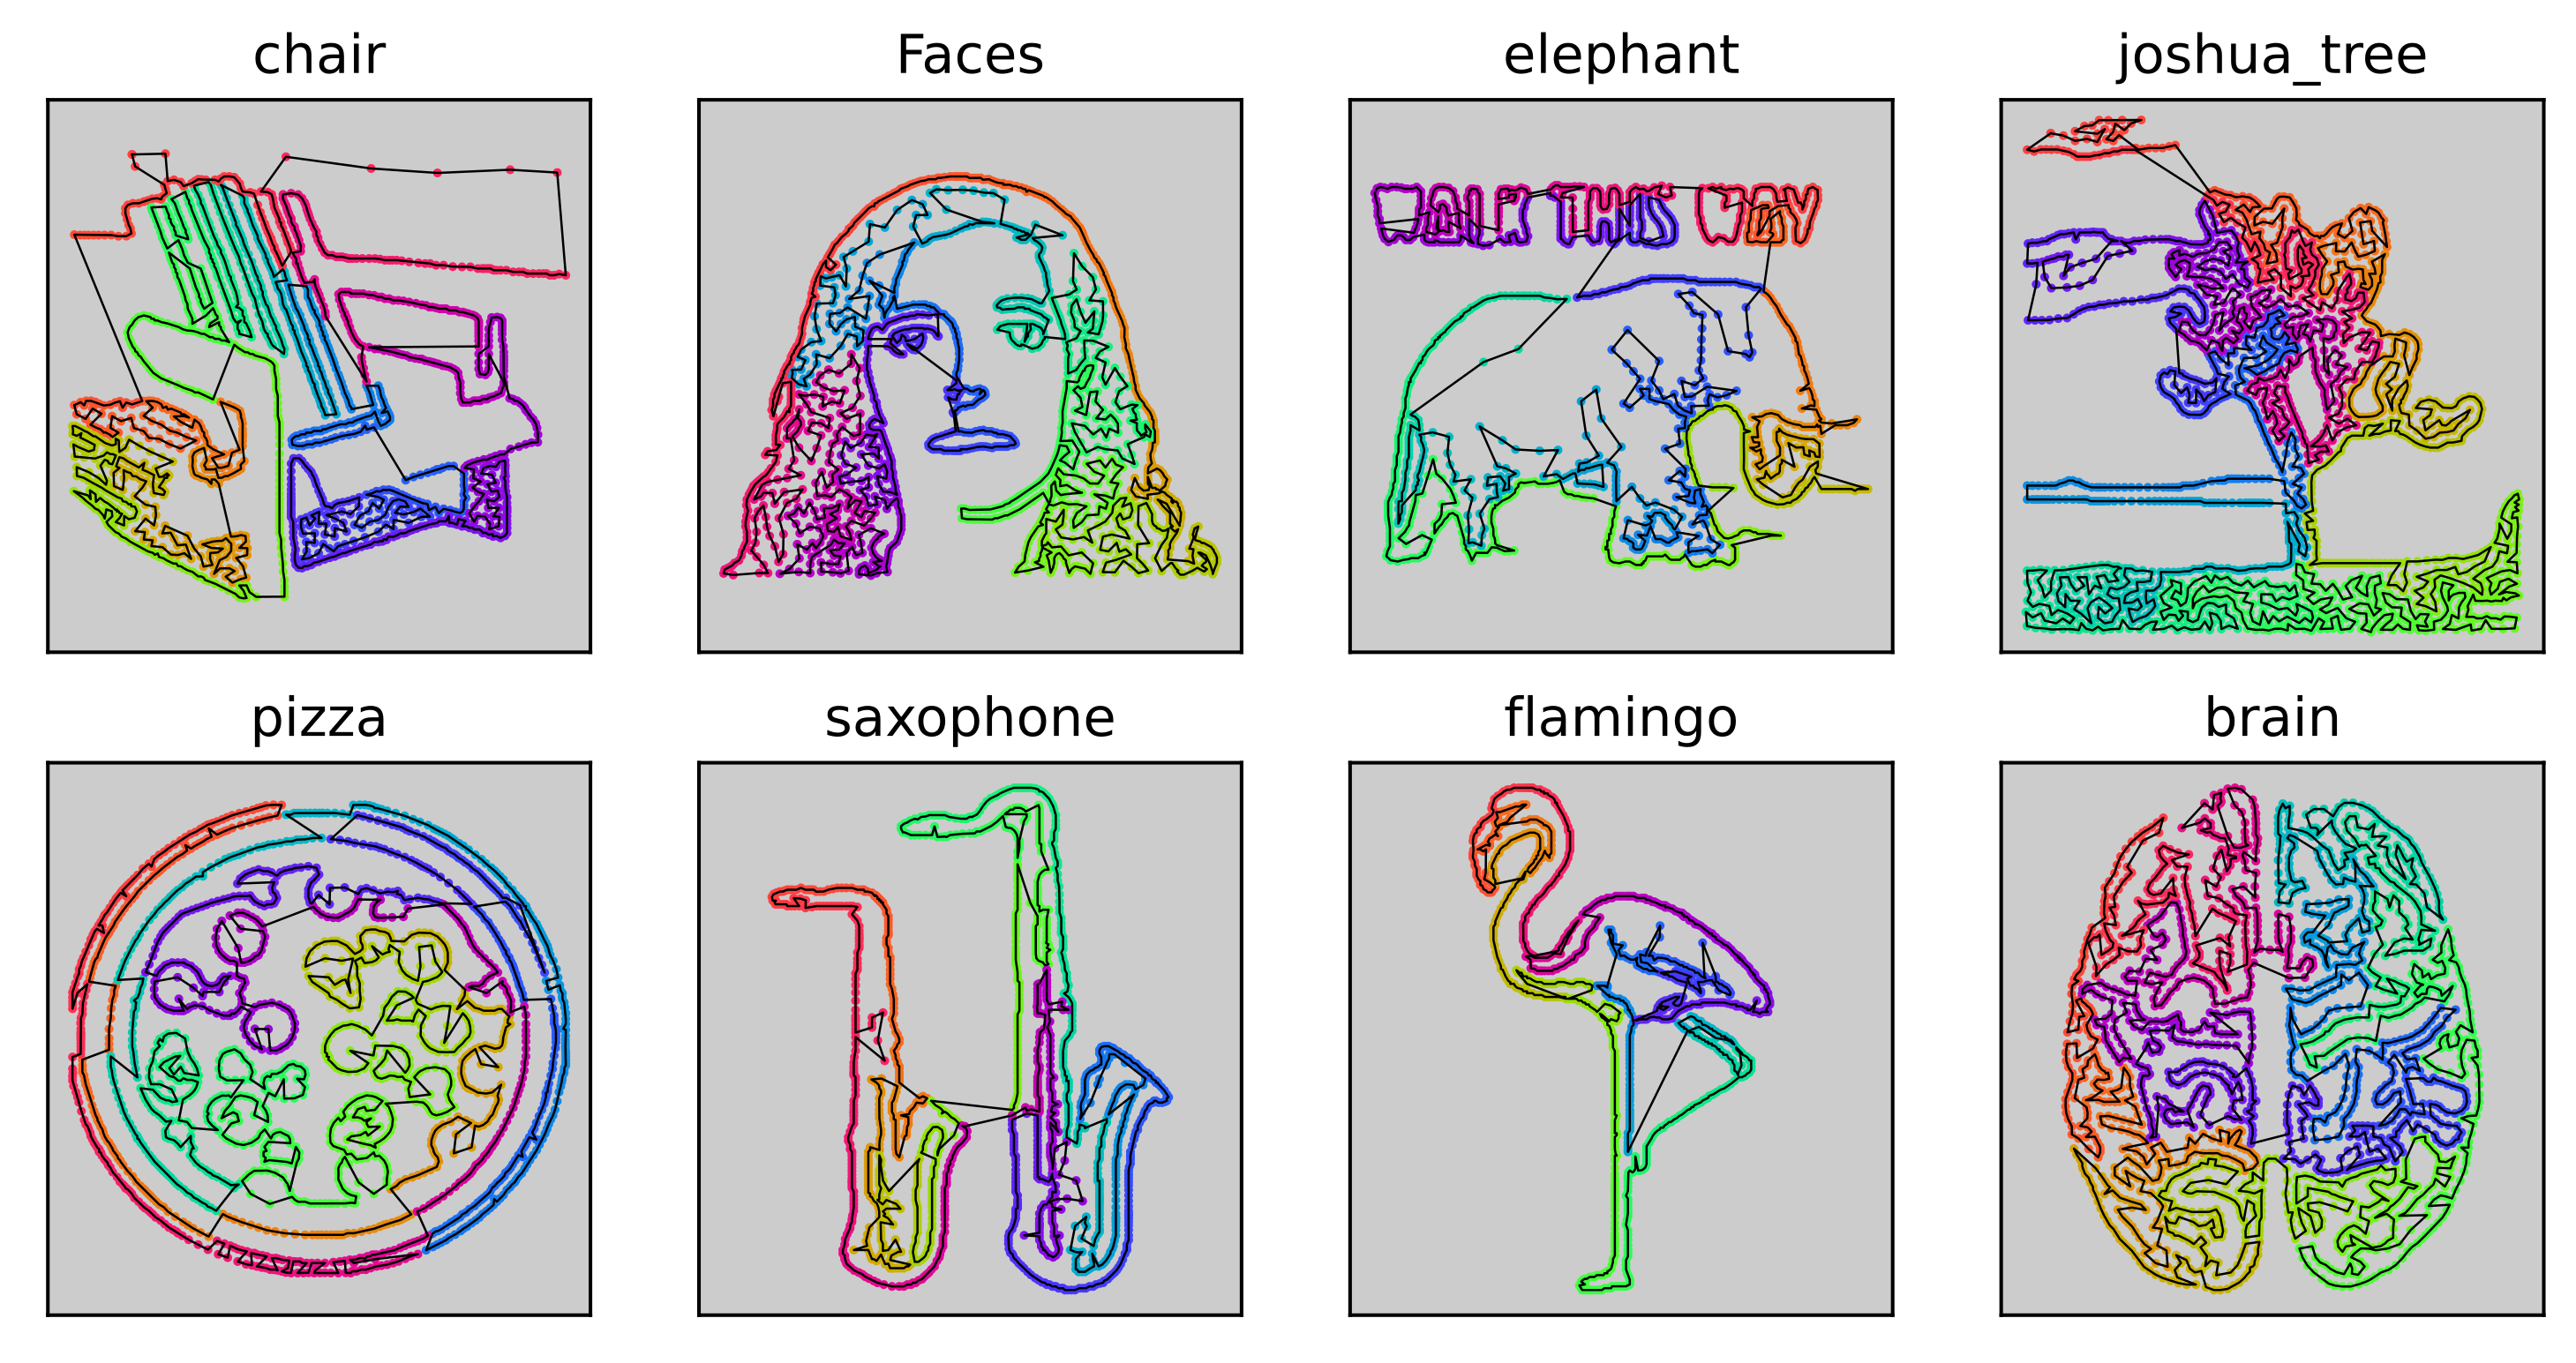
\includegraphics[width=\columnwidth]{caltech101_samples.png}
  \caption{Examples of some TSP art on the Caltech-101 dataset \cite{li_andreeto_ranzato_perona_2022}.}
  \label{fig:caltech101examples}
\end{figure}

\begin{figure}
  \centering
  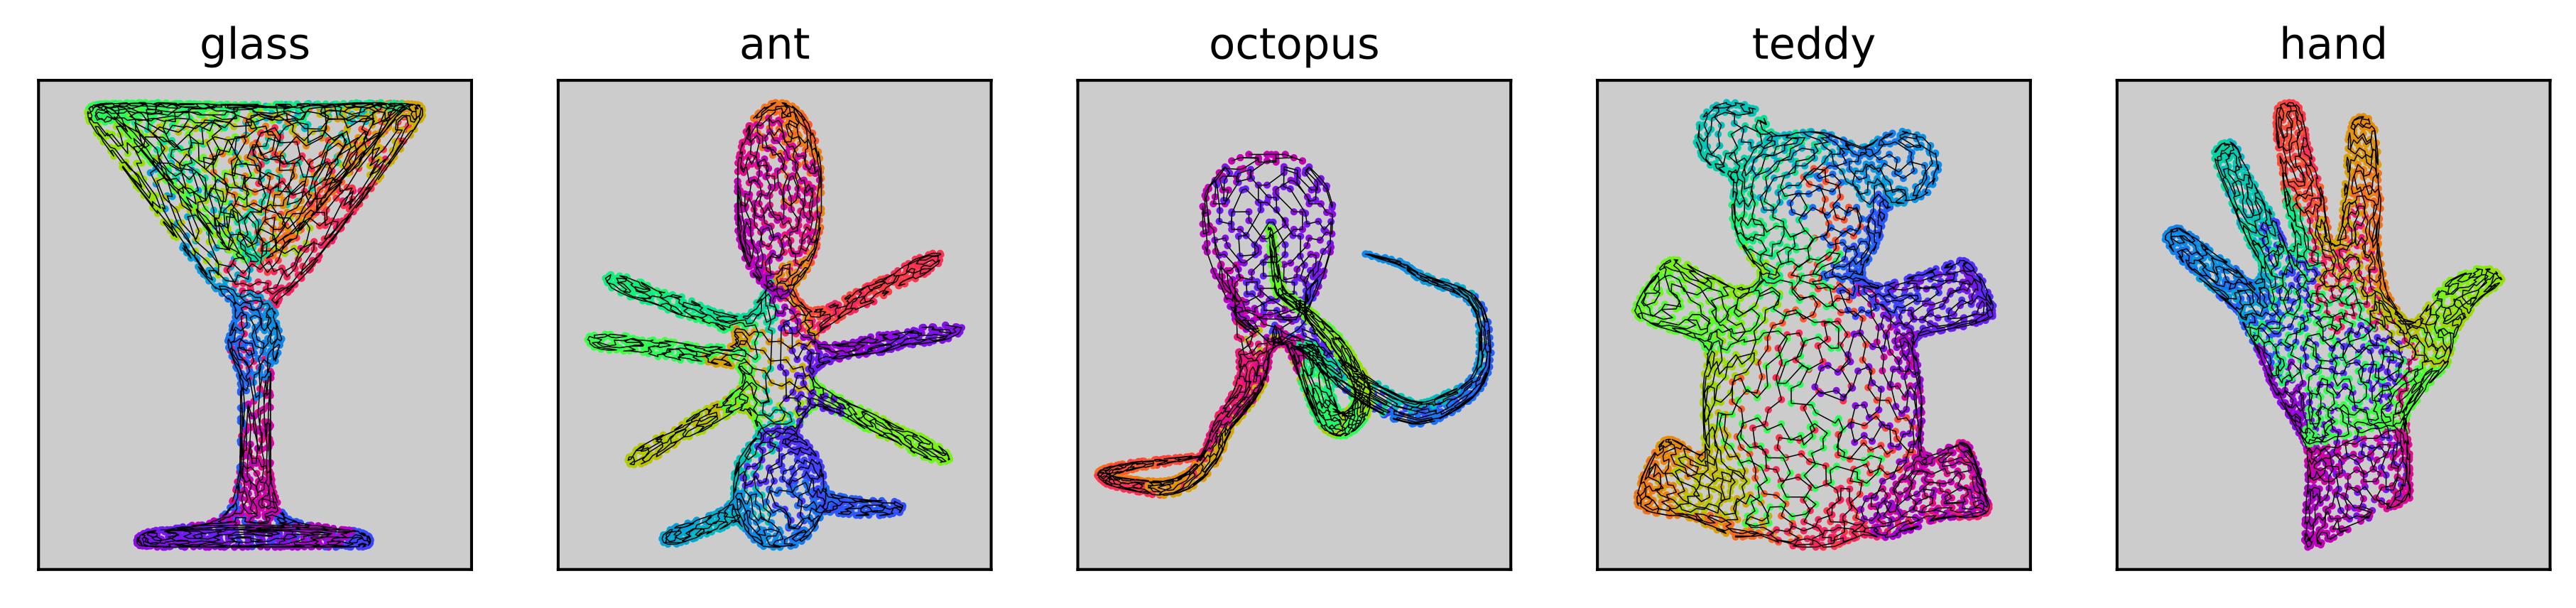
\includegraphics[width=\columnwidth]{MeshSegExamples.png}
  \caption{Examples of some Hamiltonian cycles on triangle meshes from the Princeton mesh segmentation benchmark \cite{Chen:2009:ABF}.}
  \label{fig:meshsegexamples}
\end{figure}

\subsection{Quantitative Results}


\begin{figure}
  \centering
  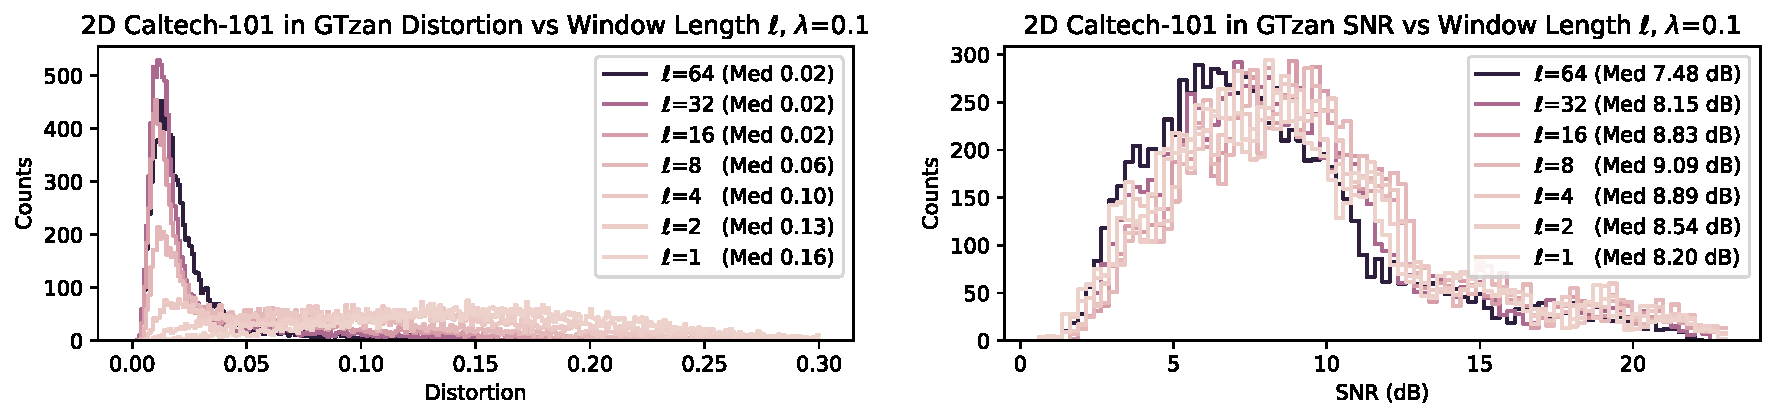
\includegraphics[width=\columnwidth]{CaltechGTzanFixedLam.pdf}
  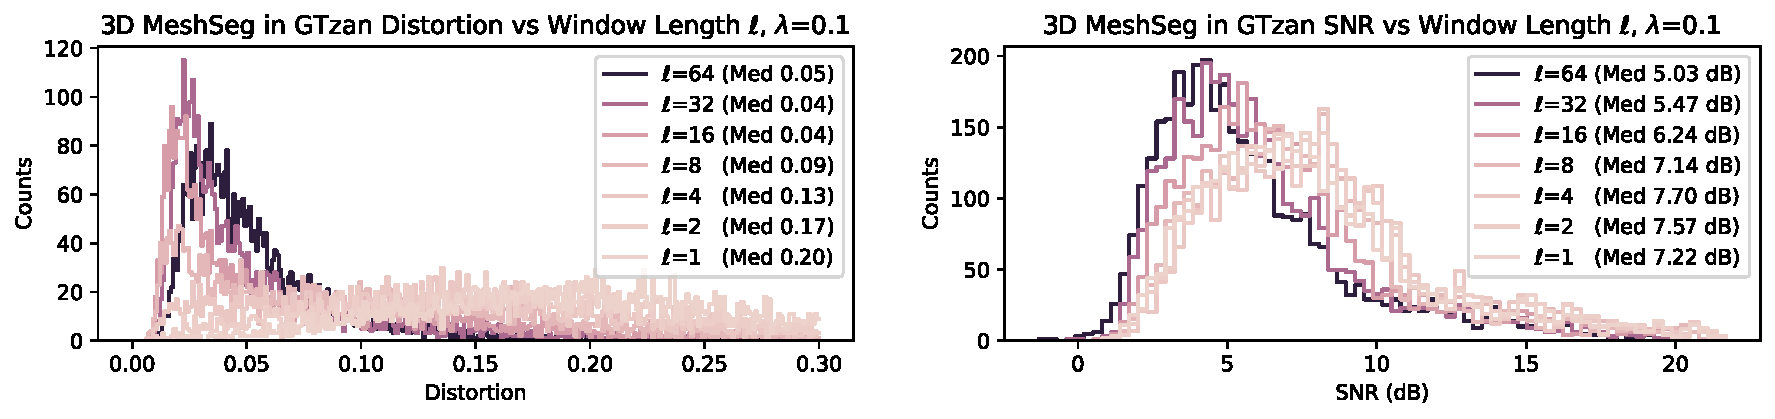
\includegraphics[width=\columnwidth]{MeshSegGTzanFixedLam.pdf}
  \caption{The results embedding curves into clips from the Tzanetakis genre dataset varying the window length $\ell$ for a fixed $\lambda$.  Moderate window lengths are the best choices for both SNR and distortion.  We recommend $\ell=16$.}
  \label{fig:ResultsFixedLam}
\end{figure}

\begin{figure}
  \centering
  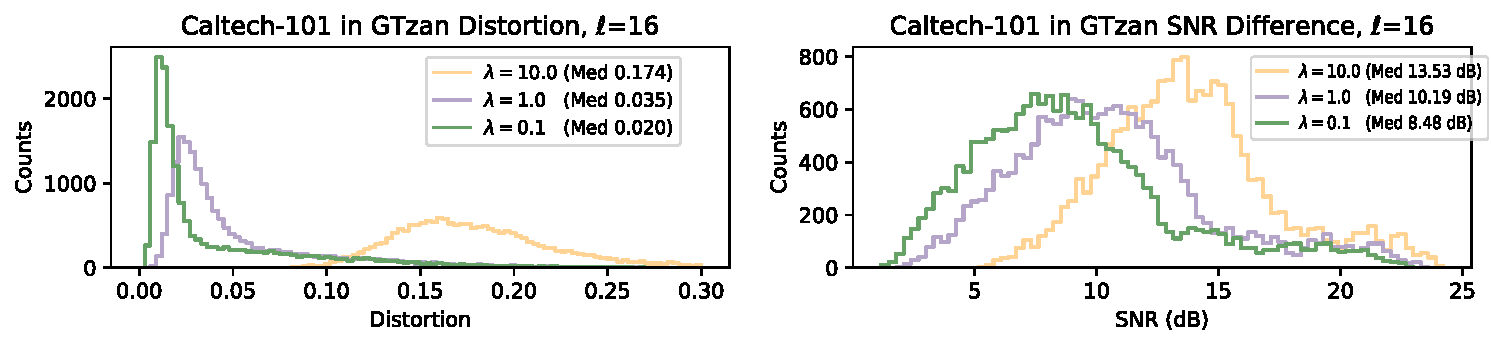
\includegraphics[width=\columnwidth]{CaltechGTzanFixedWin.pdf}
  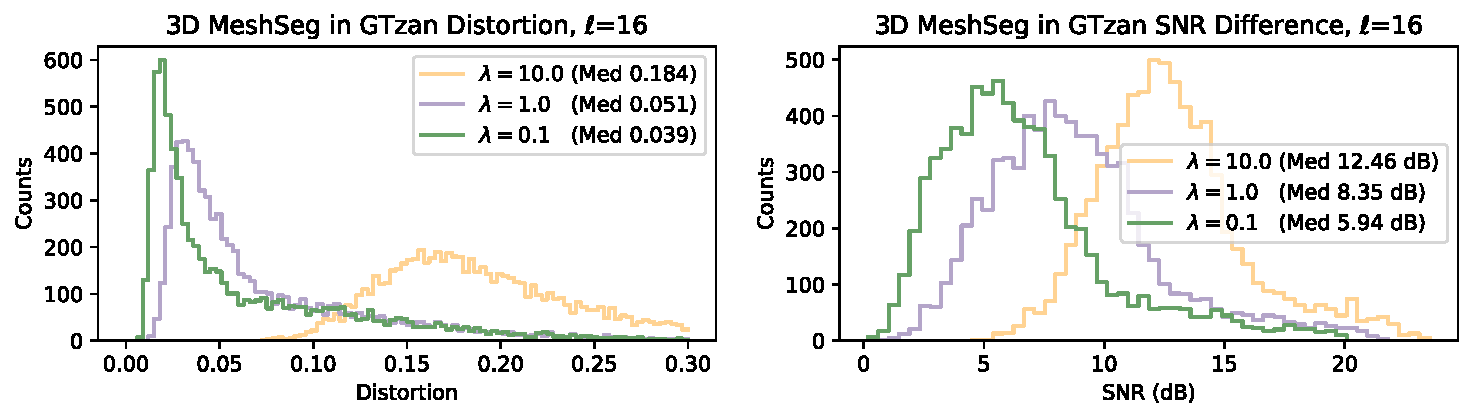
\includegraphics[width=\columnwidth]{MeshSegGTzanFixedWin.pdf}
  \caption{The results embedding curves into clips from the Tzanetakis genre dataset, for a fixed $\ell=16$.  As expected from Equation~\ref{eq:objfn}, both the distortion and SNR go up as $\lambda$ increases.}
  \label{fig:ResultsFixedWin}
\end{figure}

\begin{figure}
  \centering
  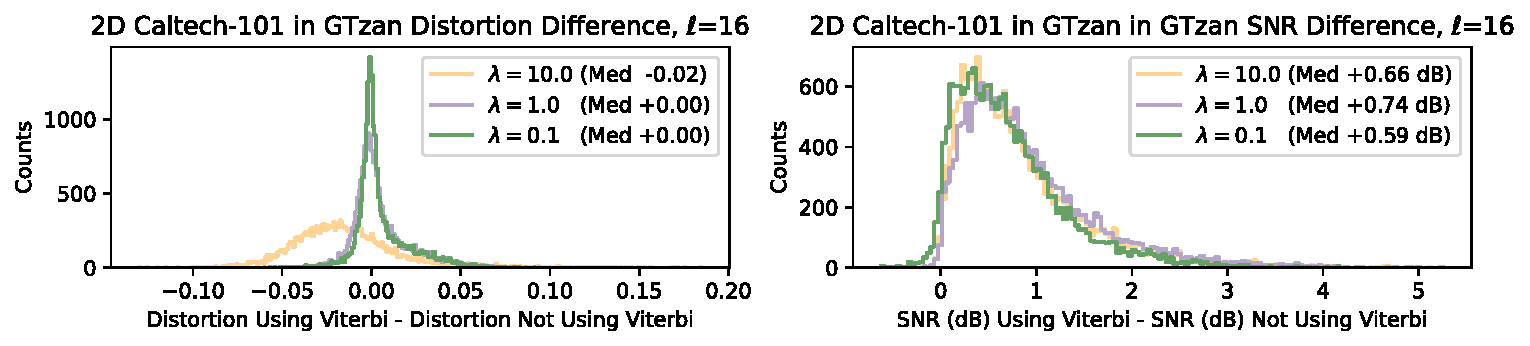
\includegraphics[width=\columnwidth]{CaltechGTzanViterbiExperiment.pdf}
  \includegraphics[width=\columnwidth]{MeshSegGtzanViterbiExperiment.pdf}
  \caption{Pre-warping the target with Viterbi alignment (Section~\ref{sec:reparam}) overall improves the resulting distortion and SNR.}
  \label{fig:ResultsViterbiExperiment}
\end{figure}

As Figure~\ref{fig:ResultsFixedLam} shows, increasing the window length has a positive effect on geometric distortion, while moderate window lengths lead to the best SNR.

\subsection{Subjective Listening Experiment}

\begin{figure}
  \centering
  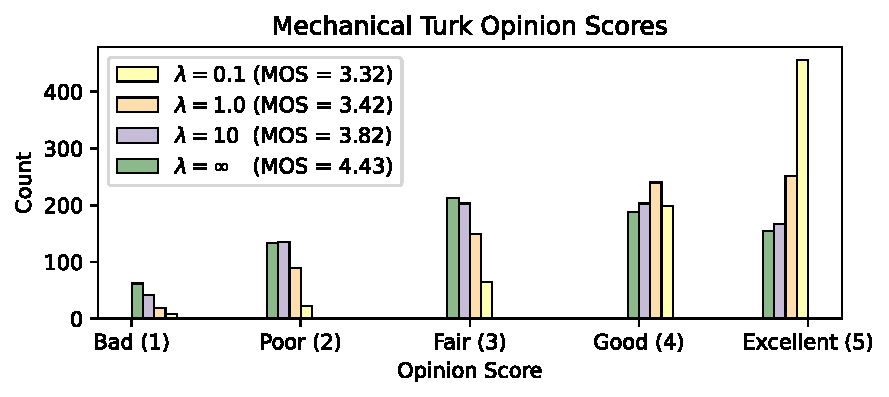
\includegraphics[width=0.8\columnwidth]{Turk.pdf}
  \caption{Results of the listening experiment on the Amazon Mechanical Turk.  A lower $\lambda$ leads to a lower mean opinion score, as expected, though not to an intolerable degree.}
  \label{fig:TurkResults}
\end{figure}


We can actually get higher SNRs using frequencies that are more audible

We ask questions similar to the authors of \cite{bassia2001robust}.

46 unique Turkers, 21 of whom participated in at least 40 rankings.

Figure~\ref{fig:TurkResults} shows the results.  Mean opinion scores are correlated with $\lambda$, but there's not much of a difference between $\lambda=0.1$ and $\lambda=1$, which suggests using the former as a rule of thumb due to its lower geometric distortion.

\section{Discussion}


Talk about how this scheme works for any orthogonal decomposition of the signal and how we tried wavelets

%
% ---- Bibliography ----
%
% BibTeX users should specify bibliography style 'splncs04'.
% References will then be sorted and formatted in the correct style.
%
\bibliographystyle{splncs04}
\bibliography{paper}
%

\end{document}

